\section{Exemples de circuits combinatoires usuels}

% =========================================================
\begin{frame}{Additionneur à propagation de retenue (RCA) : $A+B$}

    \textbf{Principe :} chaîner $n$ additionneurs complets (FA)
    en propagant la retenue $C_i$ de proche en proche
    \textbf{du LSB vers le MSB}.

    \vspace{0.2cm}

    \begin{columns}
        \begin{column}{0.45\textwidth}
            \textbf{Additionneur complet (FA) :}
            \begin{align*}
                S_i &= A_i \oplus B_i \oplus C_i \\
                C_{i+1} &= A_i B_i + (A_i \oplus B_i)\, C_i
            \end{align*}

            \textbf{Table de vérité du FA :}
            \begin{center}
              \footnotesize
              \begin{tabular}{ccc|cc}
                \toprule
                $A_i$ & $B_i$ & $C_i$ & $S_i$ & $C_{i+1}$ \\
                \midrule
                0 & 0 & 0 & 0 & 0 \\
                0 & 0 & 1 & 1 & 0 \\
                0 & 1 & 0 & 1 & 0 \\
                0 & 1 & 1 & 0 & 1 \\
                1 & 0 & 0 & 1 & 0 \\
                1 & 0 & 1 & 0 & 1 \\
                1 & 1 & 0 & 0 & 1 \\
                1 & 1 & 1 & 1 & 1 \\
                \bottomrule
              \end{tabular}
            \end{center}
        \end{column}

        \begin{column}{0.55\textwidth}
          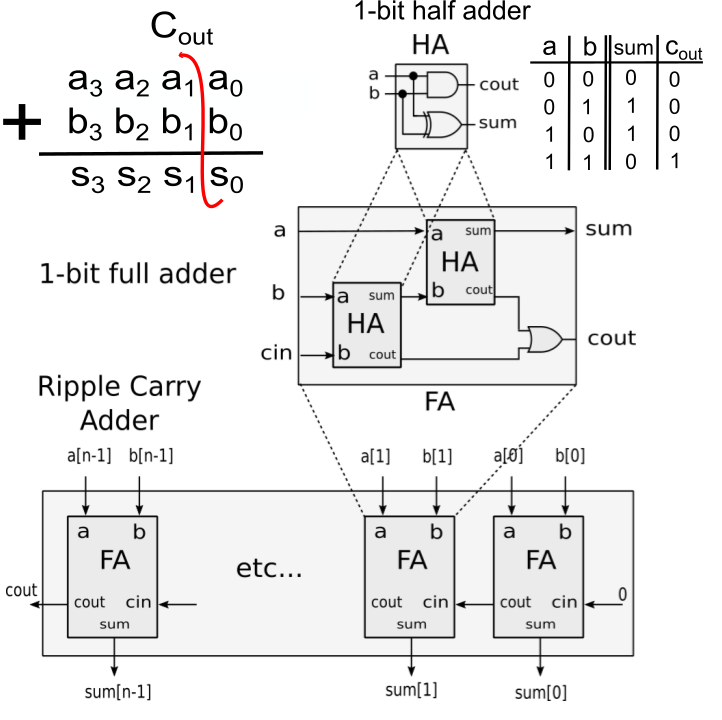
\includegraphics[scale=0.35]{./images/ripple_carry_adder.png}
        \end{column}
    \end{columns}

    %
    % \begin{block}{Point clé}
    %     \textbf{Temps critique} : $O(n)$ à cause de la propagation
    %     en cascade de la retenue (de droite à gauche). D'où les
    %     variantes plus rapides (CLA, carry-select, carry-skip).
    % \end{block}
\end{frame}

\begin{frame}{Soustracteur}
    \textbf{Principe :} réutiliser un additionneur \(n\) bits en agissant sur le second opérande via des portes \texttt{NOT} et injectant une retenue entrante.

    \vspace{0.3cm}

    \begin{columns}[T]
        \begin{column}{0.55\textwidth}
            \textbf{Idée clé :} soustraire \(B\) revient à ajouter son complément à deux :
            \[
                A - B = A + -B = A + \overline{B} + 1
            \]
        \end{column}
        \begin{column}{0.45\textwidth}
            \begin{center}
              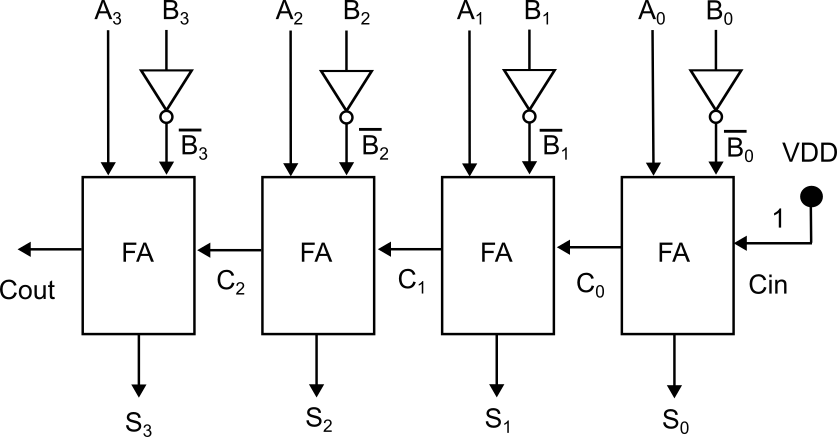
\includegraphics[scale=0.3]{./images/substractor.png}
            \end{center}
        \end{column}
    \end{columns}

    \vspace{0.2cm}
    \begin{block}{Point clé}
        Une seule porte \texttt{NOT} par bit + une retenue d'entrée à \texttt{1}: l'additionneur devient un \emph{soustracteur} sans modifier sa structure interne.
    \end{block}
\end{frame}

\begin{frame}{Additionneur-Soustracteur : un composant \textit{programmable}}
    \textbf{Principe :} réutiliser un additionneur \(n\) bits en agissant sur le second opérande via des portes \texttt{XOR} commandées par un signal \(\mathrm{sub}\) également utilisé en retenue \textit{entrante}.

    \vspace{0.3cm}

    \begin{columns}[T]
        \begin{column}{0.55\textwidth}
            \centering
            \begin{tabular}{cc|c}
              \toprule
              $B_i$ & SUB & $B_i'$ \\
              \midrule
              0 & 0 & 0 \\
              0 & 1 & 1 \\
              1 & 0 & 1 \\
              1 & 1 & 0 \\
              \bottomrule
            \end{tabular}
            \begin{itemize}
                \item \textbf{sub = 0} : \(B_i' = B_i \oplus 0 = B_i\), \(C_{in}=0\)
                \begin{itemize}
                  \item \textbf{addition} \(A+B\)
                \end{itemize}
                \item \textbf{sub = 1} : \(B_i' = B_i \oplus 1 = \overline{B_i}\), \(C_{in}=1\)
                \begin{itemize}
                  \item \textbf{soustraction} \(A-B\)
                \end{itemize}
            \end{itemize}
        \end{column}
        \begin{column}{0.45\textwidth}
            \begin{center}
              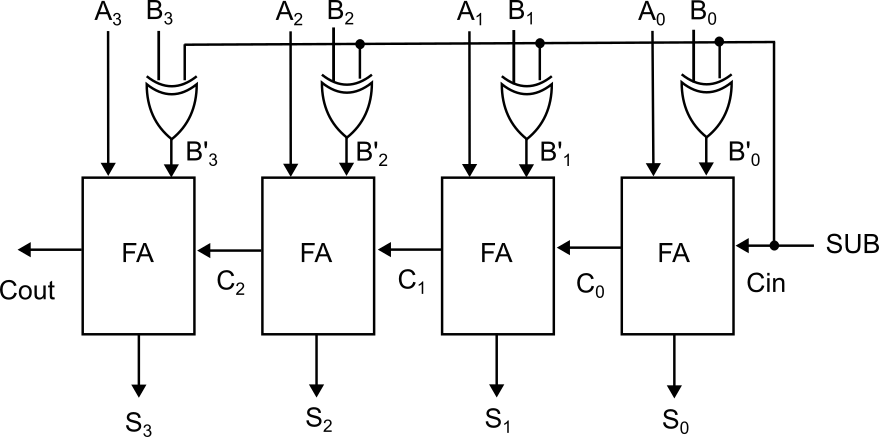
\includegraphics[scale=0.3]{./images/adder_substractor.png}
            \end{center}
        \end{column}
    \end{columns}

    \vspace{0.2cm}
    \begin{block}{Point clé}
        Une seule porte XOR par bit + une retenue d'entrée : l'additionneur devient un \emph{additionneur-soustracteur} sans modifier sa structure interne.
    \end{block}
\end{frame}
%==========================================================
\begin{frame}{Multiplieur (Mult)}

    \textbf{Principe :} suite
    d'additions décalées (algorithme « papier-crayon »).

    \vspace{0.2cm}

    \textbf{Formule booléenne (produit partiel) :}
    $PP_j = A \times b_j = A \cdot b_j \quad \text{(ET bit à bit)}$

    \textbf{Résultat :}
    $P = \sum_{j=0}^{n-1} \big( A \times b_j \big) \ll j$

    \begin{columns}
        \begin{column}{0.50\textwidth}
            \begin{center}
            \footnotesize

            \begin{tabular}{cc|c}
              \toprule
              $a_i$ & $b_j$ & $a_i \times_A b_i$ \\
              \midrule
              0 & 0 & 0 \\
              0 & 1 & 0 \\
              1 & 0 & 0 \\
              1 & 1 & 1 \\
              \bottomrule
            \end{tabular}

            \vspace{0.4cm}

            \begin{tabular}{r|cccc}
                & $a_3$ & $a_2$ & $a_1$ & $a_0$ \\
                $\times$ & $b_3$ & $b_2$ & $b_1$ & $b_0$ \\
                \midrule
                & $a_3 b_0$ & $a_2 b_0$ & $a_1 b_0$ & $a_0 b_0$ \\
                $a_3 b_1$ & $a_2 b_1$ & $a_1 b_1$ & $a_0 b_1$ & \\
                $a_2 b_2$ & $a_1 b_2$ & $a_0 b_2$ & &\\
                $a_1 b_3$ & $a_0 b_3$ & & &\\
                \bottomrule
                $p_4$ & $p_3$ & $p_2$ & $p_1$ & $p_0$ \\
            \end{tabular}
            \end{center}
        \end{column}

        \begin{column}{0.47\textwidth}
            %\footnotesize
            % \textbf{Architecture :}
            % \begin{itemize}
            %     \item $n$ portes ET (produits partiels)
            %     \item $n-1$ RCA en cascade
            %     \item Chaque RCA traite $n$ bits
            % \end{itemize}
            %
            % \vspace{0.2cm}
            % Complexité : $O(n^2)$ portes.
            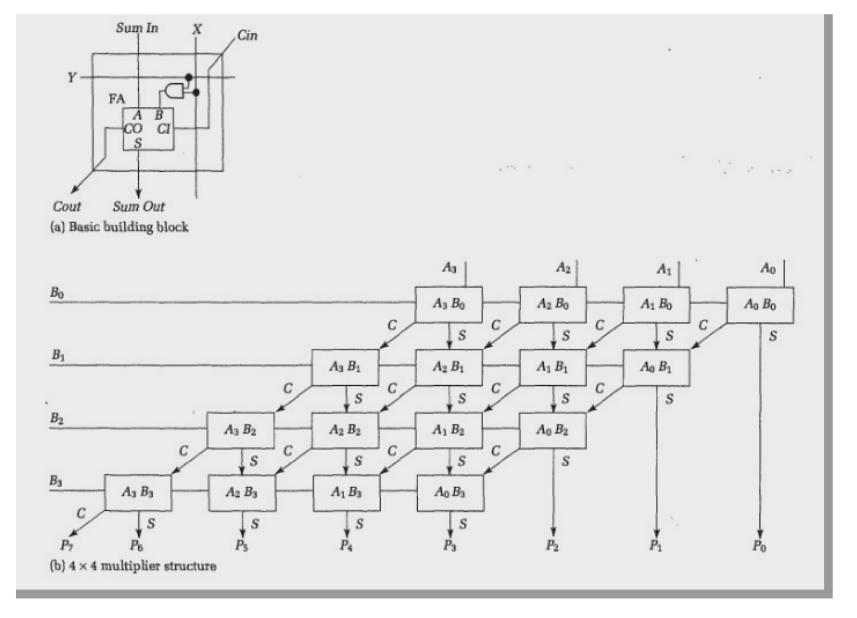
\includegraphics[scale=0.25]{./images/mult_topo.png}
        \end{column}
    \end{columns}

\end{frame}

% =========================================================
\begin{frame}{Multiplexeur 2 vers 1 (MUX21)}

    \textbf{Rôle :} sélectionner une entrée parmi deux selon un signal de commande.

    \vspace{0.1cm}

    \begin{columns}
        \begin{column}{0.5\textwidth}
          \textbf{Table de vérité :}
          \begin{tabular}{ccc|c}
                \toprule
                $A$ & $B$ & $Sel$ & $F$ \\
                \midrule
                $0$ & $0$ & $0$ & $0$ \\
                $0$ & $0$ & $1$ & $0$ \\
                $0$ & $1$ & $0$ & $0$ \\
                $0$ & $1$ & $1$ & $1$ \\
                $1$ & $0$ & $0$ & $1$ \\
                $1$ & $0$ & $1$ & $0$ \\
                $1$ & $1$ & $0$ & $1$ \\
                $1$ & $1$ & $1$ & $1$ \\
                \bottomrule
            \end{tabular}

            \vspace{0.3cm}
            \textbf{Formule booléenne :}
            $F = \overline{Sel} \times A + Sel \times B$

            \vspace{0.1cm}
        \end{column}

        \begin{column}{0.48\textwidth}
            \begin{center}
                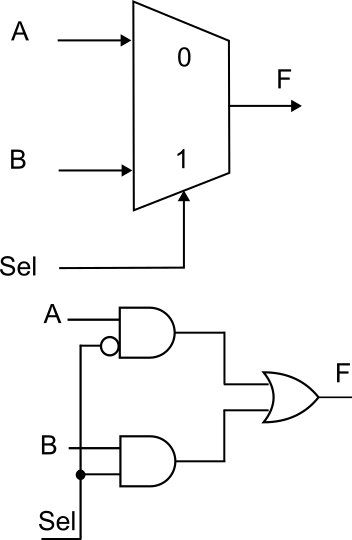
\includegraphics[scale=0.35]{./images/mux21.png}
            \end{center}
        \end{column}
    \end{columns}

    \vspace{0.1cm}

    \begin{block}{Application}
        Brique de base des MUX $2^n$→1, des barrel shifters et
        de la logique reconfigurable (FPGA).
    \end{block}

\end{frame}

% =========================================================
\begin{frame}{Shifter à position fixe (décalage par câblage)}

    \textbf{Idée clé :} décaler une donnée d'un nombre \textbf{constant}
    de positions ne nécessite \textbf{aucune porte logique}--
    un simple \textbf{recâblage} suffit.

    \vspace{0.3cm}

    \begin{columns}
        \begin{column}{0.52\textwidth}
            \textbf{Formule booléenne (décalage logique à gauche de $k$) :}
            $$S_i = \begin{cases} A_{i-k} & \text{si } i \geq k \\[2pt] 0 & \text{si } i < k \end{cases}$$

            \vspace{0.3cm}

            \textbf{Décalage logique à droite de $k$ :}
            $$S_i = \begin{cases} A_{i+k} & \text{si } i+k < n \\[2pt] 0 & \text{sinon} \end{cases}$$

            \vspace{0.3cm}

            \footnotesize Chaque sortie $S_i$ est reliée \emph{directement}
            à une entrée $A_j$ ou à la masse (0).
        \end{column}

        \begin{column}{0.46\textwidth}
            \textbf{Exemple : $A$ sur 4 bits, SLL de 1 ($k=1$)}

            \vspace{0.3cm}

            \begin{center}
            \footnotesize
            \begin{tabular}{l|cccc}
                \toprule
                Entrée A & $A_3$ & $A_2$ & $A_1$ & $A_0$\\
                \midrule
                Sortie S & $A_2$ & $A_1$ & $A_0$ & $0$ \\
                \bottomrule
            \end{tabular}
            \end{center}

            \vspace{0.3cm}

            \footnotesize Aucun composant actif : juste des fils !
        \end{column}
    \end{columns}

\end{frame}


\begin{frame}{Comparateur d'égalité de 2 mots binaires}
    \textbf{Objectif :} produire un signal \(E=1\) si et seulement si
    \(A = B\), avec \(A = A_{n-1}\dots A_0\) et \(B = B_{n-1}\dots B_0\).

    \vspace{0.2cm}

    \begin{columns}[T]
        \begin{column}{0.52\textwidth}
            \textbf{Principe :} comparer \emph{bit à bit} puis combiner.
            \[
                e_i = \overline{A_i \oplus B_i}
                \qquad (\text{XNOR})
            \]
            \[
                E = \prod_{i=0}^{n-1} \overline{A_i \oplus B_i}
            \]
            \begin{itemize}
                \item \(A_i = B_i \Rightarrow e_i = 1\)
                \item \(A_i \neq B_i \Rightarrow e_i = 0\) (et \(E=0\))
            \end{itemize}
        \end{column}
        \begin{column}{0.48\textwidth}
            \begin{center}
            \begin{circuitikz}[scale=0.5, transform shape]
                % XNOR gates (représentées par XOR + NON)
                \foreach \i/\y in {0/0, 1/-1.6, 2/-3.2, 3/-4.8} {
                    \node[xor port] (xor\i) at (0,\y) {};
                    \node[left] at (xor\i.in 1) {\(A_{\i}\)};
                    \node[left] at (xor\i.in 2) {\(B_{\i}\)};
                    \node[not port, scale=0.5] (not\i) at (2.2,\y) {};
                    \draw (xor\i.out) -- (not\i.in);
                    \node[right] at (not\i.out) {\scriptsize \(e_{\i}\)};
                }
                % AND tree
                \node[and port] (and0) at (4.8,-0.8) {};
                \node[and port] (and1) at (4.8,-4.0) {};
                \draw (not0.out) -- ++(0.3,0) |- (and0.in 1);
                \draw (not1.out) -- ++(0.3,0) |- (and0.in 2);
                \draw (not2.out) -- ++(0.3,0) |- (and1.in 1);
                \draw (not3.out) -- ++(0.3,0) |- (and1.in 2);

                \node[and port] (andF) at (7.6,-2.4) {};
                \draw (and0.out) -- ++(0.3,0) |- (andF.in 1);
                \draw (and1.out) -- ++(0.3,0) |- (andF.in 2);

                \draw[->] (andF.out) -- ++(0.8,0) node[right] {\(E\)};
            \end{circuitikz}
            \end{center}
        \end{column}
    \end{columns}

    \vspace{0.1cm}
    \begin{block}{Point clé}
        \(n\) portes \textbf{XNOR} en parallèle (une par bit) + un \textbf{ET} global
        (arbre d'AND) pour agréger les égalités partielles.
    \end{block}
\end{frame}



%============================================================
\begin{frame}{Décodeur $n \to 2^n$}
    \textbf{Principe :} Un décodeur $n \to 2^n$ active une seule sortie parmi $2^n$
    en fonction du code binaire présent en entrée.

    \vspace{0.1cm}

    \textbf{Entrées :} $A_1, A_0$ \hfill \textbf{Sorties :} $S_0, S_1, S_2, S_3$

    \vspace{0.1cm}

    \begin{columns}
        \begin{column}{0.5\textwidth}
            \textbf{Équations booléennes :}
            \begin{align*}
                S_0 &= \overline{A_1}\,\overline{A_0} \\
                S_1 &= \overline{A_1}\,A_0 \\
                S_2 &= A_1\,\overline{A_0} \\
                S_3 &= A_1\,A_0
            \end{align*}

            \vspace{0.1cm}
            Forme compacte :
            $$S_i = \prod_{k=0}^{n-1} \left( A_k \oplus \overline{b_{i,k}} \right)$$

            \vspace{0.05cm}
            \footnotesize où $b_{i,k}$ est le $k$-ième bit de la
            représentation binaire de l'indice $i$.
        \end{column}

        \begin{column}{0.48\textwidth}
            \textbf{Tableau de principe :}
            \begin{center}
                \begin{tabular}{cc|cccc}
                    \toprule
                    $A_1$ & $A_0$ & $S_0$ & $S_1$ & $S_2$ & $S_3$ \\
                    \midrule
                    0 & 0 & \textbf{1} & 0 & 0 & 0 \\
                    0 & 1 & 0 & \textbf{1} & 0 & 0 \\
                    1 & 0 & 0 & 0 & \textbf{1} & 0 \\
                    1 & 1 & 0 & 0 & 0 & \textbf{1} \\
                    \bottomrule
                \end{tabular}
            \end{center}

            \vspace{0.3cm}
            \footnotesize\textbf{Exemple :} pour $i=2$, on a
            $(b_{2,1}\,b_{2,0})_2 = (10)_2$, donc
            $b_{2,1}=1$ et $b_{2,0}=0$.
        \end{column}
    \end{columns}
\end{frame}


\begin{frame}{Décodeur BCD vers afficheur 7 segments}
  \begin{center}
      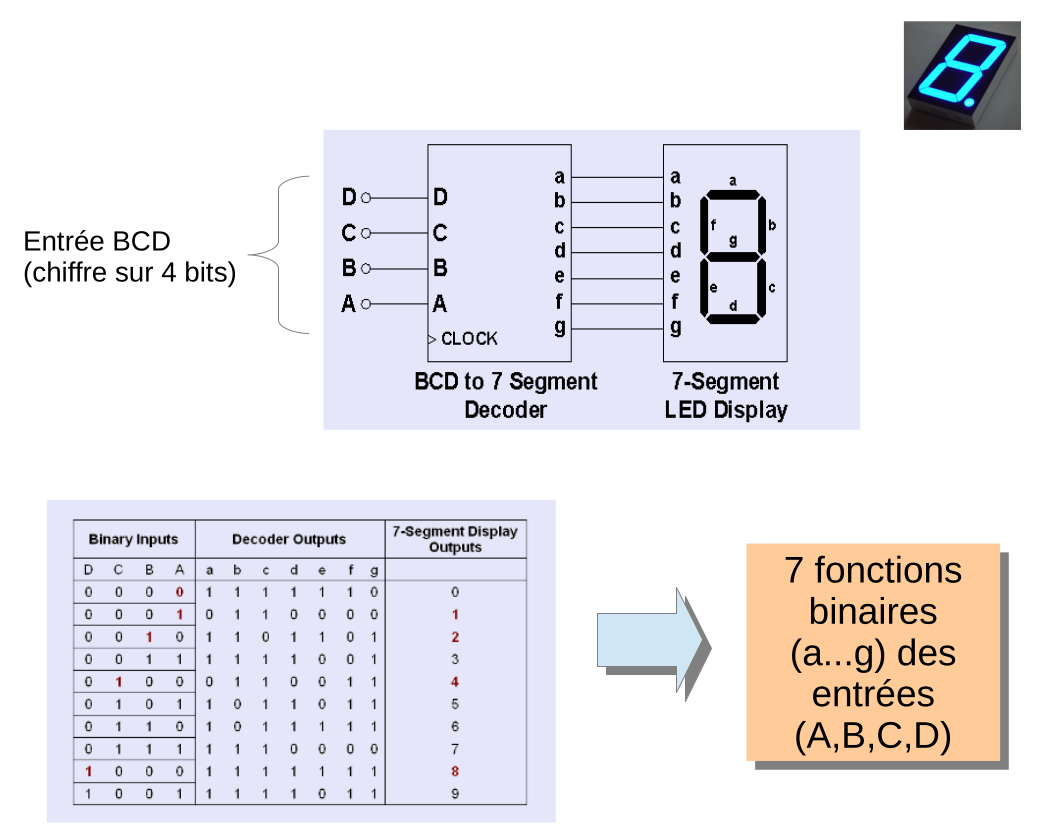
\includegraphics[scale=0.25]{./images/decoder_7seg.png}
  \end{center}
\end{frame}
